\chapter{Asking Luxury Shoppers How They Got RICH! (Miami)}

This School of Hard Knocks lecture, preserved here with curation by LazyingArt LLC, has no blackboard and no validated on-screen mathematics, but it nevertheless unfolds with a clear quantitative order. The interviewer keeps returning to the same variables---industry, yearly income, ownership, assets under management, reinvestment, delegation, and the route to financial freedom---until a common structure emerges across very different lives. We shall follow that order closely, and where a compact formula clarifies the spoken logic, we will introduce it explicitly as editorial notation rather than as visible lecture mathematics.

\section{Teaser, Method, and the Scale of the Problem}

The episode begins with a teaser montage. Before we know any mechanism, we are handed magnitudes: one guess of \$750{,}000, one answer of \$8 million, another answer of more than \$2 million, a move from construction to commercial real estate, and a report of assets under management near a billion dollars. The point is not yet to explain; the point is to load the variables.

A compact way to collect the numerical horizon of the teaser is
\begin{equation}
Y_{\max}^{\text{teaser}} \in \left\{7.5\times 10^5,\ >2\times 10^6,\ 8\times 10^6\right\}\,\mathrm{USD},
\qquad
M_t \approx 10^9\,\mathrm{USD}.
\end{equation}

We should notice the sequence of prompts attached to those values. What industry did you choose? Are you a business owner? How much do you manage? What is the blueprint for becoming financially free? The lecture is telling us, even before the formal setup in Miami, that it will proceed by repeated interrogation of a small set of economic variables.

Then the method is stated plainly. We are in the Miami fashion district, asking multimillionaires and luxury shoppers how they became successful. The luxury setting is therefore not the thesis. It is the testing ground. The lecturer first establishes scale, then sends us into cases.

\section{The Surgeon: From Profession to Ownership}

The first full case is the surgeon, and the ordering is exact. We do not begin with money. We begin with vocation. He went into healthcare; he was very close to his grandmother; he saw a surgeon when he was eight years old; that became a turning point; and only then does the lecture ask for the largest single-year income.

The answer is ``in excess of two million,'' but the speaker immediately prevents a false reading. He says the number did not arise simply because surgeries themselves paid at that level. It arose because he owned surgery centers, owned part of the place where the work was being done, built a network of orthopedic walk-in centers, and owned the real estate beneath the enterprise.

We can summarize the mechanism by introducing a bookkeeping identity:
\begin{equation}
Y_t = Y_t^{\text{labor}} + Y_t^{\text{own}} + \Delta A_t.
\end{equation}
Here \(Y_t^{\text{labor}}\) is compensation for doing the work, \(Y_t^{\text{own}}\) is the flow that comes from owning the platform on which the work is done, and \(\Delta A_t\) records the gain associated with productive assets, especially real estate.

The speaker's language is plain, but its structure is almost algebraic. If one is only an employee, then one receives
\begin{equation}
Y_t^{\text{employee}} = Y_t^{\text{labor}}.
\end{equation}
If one is instead an owner-operator, then one receives
\begin{equation}
Y_t^{\text{owner}} = Y_t^{\text{labor}} + Y_t^{\text{own}} + \Delta A_t.
\end{equation}
The ceiling changes because the margin no longer departs entirely to the institution above the worker.

\subsection{Question \& Answer}

Why does ownership break the ceiling that labor alone often cannot?

The surgeon's answer is not abstract. If one works for a large firm, the firm makes money off one's effort. That may still be a perfectly reasonable arrangement for someone who does not want the burden of business headaches. But it means that the margin sits elsewhere. Once one owns the practice, the center, the network, and the building, the same skill is now embedded in a larger balance sheet.

That is why this interview becomes the first genuine mechanism in the lecture. It is not a generic celebration of entrepreneurship. It is a specific claim that ownership of the operating platform changes the decomposition of income.

A second move follows naturally. Once the lecture has shown us how large flows can be generated, it asks how those flows are to be treated. The surgeon answers with the power of compounding interest and with a warning against premature extravagance. In a place like this, surrounded by luxury, one may eventually splurge. But when one is younger, one should be judicious.

The update rule suggested by that advice is
\begin{align}
W_{t+1} &= (1+r_t)W_t + S_t,\\
S_t &= Y_t - C_t,\\
C_t &= C_t^{\text{needs}} + C_t^{\text{wants}}.
\end{align}
Here \(W_t\) is investable wealth, \(r_t\) is the return earned by existing wealth, \(S_t\) is the new amount added out of current income, and consumption is split into what one must cover and what one merely desires.

\paragraph{Worked derivation.}
If we freeze the return and the contribution, so that \(r_t=r\) and \(S_t=S\), then the compounding logic can be unfolded explicitly:
\begin{align}
W_1 &= (1+r)W_0 + S,\\
W_2 &= (1+r)W_1 + S = (1+r)^2W_0 + \bigl[(1+r)+1\bigr]S,\\
W_3 &= (1+r)W_2 + S = (1+r)^3W_0 + \bigl[(1+r)^2+(1+r)+1\bigr]S.
\end{align}
By induction one obtains
\begin{equation}
W_n = (1+r)^n W_0 + S\sum_{j=0}^{n-1}(1+r)^j
     = (1+r)^n W_0 + S\frac{(1+r)^n-1}{r},
\end{equation}
provided \(r\neq 0\). The lecture never writes this formula, but it is the clean standard form of the spoken advice: invest early, keep contributing, and let the old money work on the new.

Since no validated lecture diagram survives, the following figure is an editorial schematic of the recurring ladder already implicit in the surgeon's case.

\begin{figure}
\centering
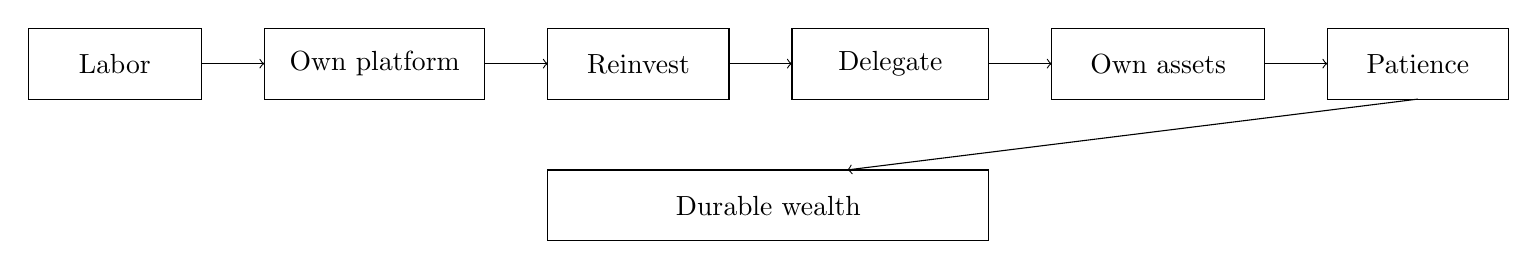
\begin{tikzpicture}[x=1cm,y=1cm]
\draw (0,0) rectangle (2.2,0.9);
\node at (1.1,0.45) {Labor};

\draw[->] (2.2,0.45) -- (3.0,0.45);

\draw (3.0,0) rectangle (5.8,0.9);
\node at (4.4,0.45) {Own platform};

\draw[->] (5.8,0.45) -- (6.6,0.45);

\draw (6.6,0) rectangle (8.9,0.9);
\node at (7.75,0.45) {Reinvest};

\draw[->] (8.9,0.45) -- (9.7,0.45);

\draw (9.7,0) rectangle (12.2,0.9);
\node at (10.95,0.45) {Delegate};

\draw[->] (12.2,0.45) -- (13.0,0.45);

\draw (13.0,0) rectangle (15.7,0.9);
\node at (14.35,0.45) {Own assets};

\draw[->] (15.7,0.45) -- (16.5,0.45);

\draw (16.5,0) rectangle (18.8,0.9);
\node at (17.65,0.45) {Patience};

\draw (6.6,-1.8) rectangle (12.2,-0.9);
\node at (9.4,-1.35) {Durable wealth};

\draw[->] (17.65,0) -- (10.4,-0.9);
\end{tikzpicture}
\end{figure}

The first serious lesson of the lecture is therefore already complete. High income is not denied. But high income is no longer the main variable. The deeper variable is the structure within which the income is generated and then preserved.

\section{Street Reset, Luck, and the Cost of Growth}

At this point the lecture deliberately relaxes. There is a fan interaction, a burst of thank-yous, and a street-level reset. That material is not incidental. It clears the emotional space after a dense first interview and prepares us for a more uneven sequence of entrepreneurial voices.

The next surviving fragment is slightly garbled, but its direction is clear. One speaker says he got lucky. He would like to say he was brilliant and researched his way there, but instead he tells a more opportunistic story: he went to a seminar, saw a product, saw a market need, noticed nobody was doing it, and took a chance. The maxim that follows is wonderfully rough: one does not hit a home run without taking many swings.

We then hear the line, ``finance isn't about math, it's about choices.'' That should not be read as an anti-mathematical slogan. It is a statement about decision order. The lecture's earlier split between \(C_t^{\text{needs}}\) and \(C_t^{\text{wants}}\) now receives its crispest verbal form: deal with what is necessary first, then move outward.

The contractor case sharpens this from life advice into operating advice. He has been in the industry for twenty-seven years, starting with his father, and says that consistent sales came from producing a perfect product. If the work is good enough, clients find you. But he couples this with another principle that sounds reckless only if we detach it from the business setting: you have to spend money to make money.

We can formalize that mechanism cautiously as
\begin{equation}
K_{t+1} = K_t + I_t - \delta K_t,
\end{equation}
where \(K_t\) is productive business capacity, \(I_t\) is reinvestment into that capacity, and \(\delta K_t\) is wear, drift, or obsolescence.

The contractor then explains what \(I_t\) means in practice: better tools, better labor, and a stronger team. So the real claim is not indiscriminate spending. It is that some expenditure is not consumption at all. It is a transfer from current cash into future productive power.

We may organize the logic as follows:
\begin{enumerate}
\item Surplus that is consumed immediately vanishes into \(C_t\).
\item Surplus redirected into \(I_t\) enlarges \(K_t\).
\item Higher \(K_t\) raises what the business can promise and what it can reliably deliver.
\item Better delivery reinforces reputation and future revenue.
\item Future revenue funds the next round of reinvestment.
\end{enumerate}

This is one of the lecture's most useful corrections. Earlier the surgeon warned us against excessive spending. Here the contractor warns us against confusing austerity with growth. The two claims are not contradictory. They sort spending into categories: status consumption is one thing, productive reinvestment another.

\section{Finance at Scale: Delegation, Risk Narratives, and Sales}

The next clean case is finance in the direct, operational sense: mortgage, personal loans, credit cards. ``We lend out money,'' the speaker says. He has been in business for about twenty years, always wanted to be his own boss, and reports a single-year income of about \$8 million. The lecture now asks the central scale-up question as explicitly as it ever does: what does a six-figure person need in order to move to seven figures?

\subsection{Question \& Answer}

The answer is delegation.

The speaker certainly says to work hard, but that is not the new idea. The new idea is that one must learn to trust other people to do the job. The founder who says ``I can do it myself'' is defending competence at the cost of scale.

A compact reconstruction of that logic is
\begin{equation}
Q_t = q(K_t,n_t),
\qquad
\frac{\partial q}{\partial K}>0,
\qquad
\frac{\partial q}{\partial n}>0.
\end{equation}
Here \(Q_t\) is effective business throughput, \(K_t\) is productive capacity, and \(n_t\) is effective team span. The inequalities merely record the directional claim spoken in the interview: more capable infrastructure and a larger trusted team expand the size of the operation.

At fixed founder hours, the solo ceiling is binding. Delegation relaxes that ceiling. The lecturer's question is therefore answered not by a motivational slogan but by an operational one: move from personal effort to organized effort.

The interview then widens to investment. The speaker strongly recommends cryptocurrency and frames the issue as one of control: when money sits in a bank, the bank controls it; when value is held in crypto, the holder controls it more directly.

\begin{remark}
We preserve this as the speaker's risk narrative, not as settled doctrine. The lecture's real content here is the contrast between delegated custody and direct control. The numerical insurance threshold and the legal absolutes that accompany the claim should be handled cautiously in any later polished version.
\end{remark}

The lecturer then pivots again, asking not where money should go, but how clients are won and kept.

\subsection{Question \& Answer}

How does one consistently land clients throughout a career?

The answer is that sales is not a narrow niche inside business. It is the universal layer beneath business. A doctor sells, an attorney sells, a dentist sells, and every human interaction in economic life contains some act of persuasion, framing, or trust formation.

What is especially good here is that the speaker does not end in abstraction. He gives a training rule: go into the company, find the top producer, and sit next to that person. The lecture has therefore moved from a very large claim---everything is a sale---to a very local prescription---learn in the orbit of the person who is already best at it.

This is one of the recurring motifs of the entire chapter. Do not merely admire success from a moral distance. Put yourself close enough to watch the operating procedure.

\section{Career Capital, Packages, and Institutional Apprenticeship}

A sponsor break interrupts the interviews. We should mark it as a structural pause rather than as part of the lecture's core doctrine. Its themes are time, food, and routine: the entrepreneur is always moving, and wasted time has an opportunity cost. Then the lecture returns, but now on a slower and more institutional register.

The hospitality speaker has spent twenty years getting into his present position. He is now part partner or a minority stakeholder in a brand, yet he insists that this does not reduce the quantity of work. On the contrary, the real work begins where others think it ends. The sale is not the end. Ownership extends the chain of responsibility.

This case is important because it widens the concept of capital. The speaker worked for Louis Vuitton and other French conglomerates before arriving at his present role. He advises the listener not simply to compare salaries, but to inspect the whole package: features, benefits, room for growth, equity, and, crucially, the quality of the boss.

A more faithful summary of this than a simple income formula is an offer-value decomposition:
\begin{equation}
V^{\text{package}}
=
V^{\text{cash}}
+
V^{\text{growth}}
+
V^{\text{equity}}
+
V^{\text{learning}}.
\end{equation}
The last term matters enormously in this interview. The speaker says he worked with industry titans and multiple billionaires, and that the experience gained from those people could not be replicated in a lifetime by ordinary means.

So the lecture is now teaching us to evaluate a trajectory, not merely a paycheck. A high-quality position may be valuable because it offers
\begin{itemize}
\item current cash compensation,
\item internal opportunities for growth,
\item access to equity or ownership,
\item apprenticeship under unusually capable people.
\end{itemize}

The case therefore extends an earlier theme. In the surgeon's story, ownership sat above skill. Here, institutional apprenticeship sits before ownership. We do not simply leap to the top of the ladder. Sometimes we spend twenty years learning how the upper floors are built.

\section{Todd Napola: Patience, Class Scripts, and the Blueprint}

The lecture then announces a special surprise and shifts into its capstone interview with Todd Napola. The scale changes again. We are told he manages over a billion dollars of property and runs one of the largest commercial real estate companies in South Florida. The lecture also tells us how to read that scale: not as a reason for awe, but as a reason to listen carefully to the next few organizing principles.

\begin{equation}
M_t \approx 10^9\,\mathrm{USD}.
\end{equation}

Napola says he began in finance, moved into real estate for financial independence, and now lives at a horizon quite unlike the daily horizon of quoted equities. That point deserves its own notation, modest though it is:
\begin{equation}
H_{\mathrm{RE}} \gg 1\ \text{day},
\end{equation}
where \(H_{\mathrm{RE}}\) denotes the relevant holding and decision horizon in real estate. The lecture's point is that real estate should not be read as though it were a brokerage screen to be checked every afternoon. Values move, but the governing timescale is longer, often much longer.

This is why patience becomes the master word of the interview. The richest real-estate families appear generational because they began buying generations ago. But the lesson drawn is not passive admiration for old money. It is that somebody had to begin the sequence. One must be the one who starts now.

The lecture then makes its broadest social move and asks about the difference between the middle class and the wealthy. Napola's answer is severe. He says the middle class got trapped inside an inherited script that once sounded prudent and now no longer works. In compressed form, that script is
\begin{itemize}
\item go to school,
\item get a good job,
\item save money,
\item buy a house,
\item pay it off,
\item retire on a pension.
\end{itemize}
His claim is not that each step is irrational in isolation. It is that the whole script presupposes a world that has already changed. The lecture has now arrived at its strongest external diagnosis: a large part of the population is still using a map drawn for another economic landscape.

\subsection{Question \& Answer}

What, then, is the blueprint for becoming a millionaire and getting serious about financial freedom?

Napola's answer is the cleanest synthesis of the lecture. Work hard to add value to other people. Put yourself near wealthy people, not to imitate their consumption, but to discover that they are not ontologically different from you. Then watch where value is actually being created and model people who built from the bottom rather than inheriting a final form.

His valet-at-the-country-club example is useful precisely because it is so concrete. A talented salesperson who believes rich people are a different species is still trapped in a false cosmology. Put him in a place where he parks their cars, hears their jokes, and sees their mannerisms, and the superstition dissolves. The economic question can finally replace the psychological one.

We may therefore write the blueprint as a sequence rather than as a slogan:
\begin{enumerate}
\item remove the false transcendence of wealth;
\item identify where real value can be added;
\item stay near people who already allocate capital and opportunity at scale;
\item choose ownership structures and horizons that allow that value to accumulate.
\end{enumerate}

This does not make the road easy. Napola explicitly says the person without privilege may have to work much harder. But the lecture's conclusion is that difficulty is not impossibility. The path exists, and the task is to identify its operative variables correctly.

\section{Summary}

The lecture begins with spectacle, but it does not remain there. One by one, the interviews turn headline numbers into mechanisms. The surgeon teaches us that labor alone is not the whole income process; ownership of the platform and the asset changes the decomposition. The middle cases teach us that luck, repeated attempts, and reinvestment matter; that productive spending is not the same as frivolous consumption; and that scale requires delegation rather than heroic self-containment. The later cases add institutional apprenticeship, package quality, and long-horizon patience.

If we compress the entire chapter into one statement, it is this: wealth becomes durable when skill is joined to ownership, surplus is joined to compounding and reinvestment, growth is joined to delegation, and the whole process is allowed to unfold on a timescale longer than daily noise.